\chapter{引言}
%引言是论文正文的开端,应包括毕业论文选题的背景、目的和意义;
%对国内外研究现状和相关领域中已有的研究成果的简要评述;
%介绍本项研究工作研究设想、研究方法或实验设计、理论依据或实验基础;
%涉及范围和预期结果等。要求言简意赅,注意不要与摘要雷同或成为摘要的注解。
\label{cha:introduction}
\section{选题背景与意义}
\label{sec:background}
近年来,人工智能技术快速发展,日新月异。复杂多变的环境对人工智能技术
提出了更高的要求,更加智能的算法成为了人们的追求。
从周围环境中获取准确信息是智能体对周围环境做出决策的基础,其中深度估计,
即获得环境与智能体之间的距离信息,对于智能体来说十分重要。
尤其对三维重建,3D物体检测,即时定位与建图等任务更是不可或缺的步骤。
在深度估计算法中,传感器感知算法使用传感器依靠环境对自身释放信号
的反馈来获取信息,例如通过雷达扫描获得点云数据进而预测深度。
其优点是较为精确,算法稳定不易受到环境干扰。但是存在数据稀疏,
设备成本高的问题。广泛使用的还有双目立体匹配算法,模拟了生物的双眼,
通过对双目相机获取的图像进行立体匹配,从而获得双目视差信息,进一步依靠基线
和几何知识可获得深度信息。但是,双目相机完全同步较为困难,
且对硬件条件(相机相对位置,绝对位置,
相机内参外参等)要求较为严格。
单目深度估计即从一张给定的RGB图像中恢复出图像中的场景到
相机的距离,并存储在深度图像素中。该问题可以被描述为:
给定一个集合$\mathcal{T} = \{(I,D)\}$, 
$I\in \mathcal{I}$, $D\in \mathcal{D}$,
其中$\mathcal{I}$和$\mathcal{D}$分别是RGB图像和真实深度图集合,
算法希望获得从$\mathcal{I}$到$\mathcal{D}$的映射
$\varPhi : \mathcal{I} \rightarrow \mathcal{D}$. 

单目深度估计算法相比传感器和双目深度估计具有独特的的优势:
对硬件要求较低,
采集单目RGB图像的相机可以是消费级。
基于这些优势,近年来学者们对单目深度估计算法进行了深入的研究。
但是单目深度估计算法也有其不可忽视的缺点:
场景的3D信息在图像采集过程中完全丢失,因此,要恢复已损失的深度信息,
算法需要拟合的映射$\varPhi$缺乏理论依据,
这使得算法实现具有一定难度。但是随着深度学习技术的不断进步,
数据在多样性和数量上得到了极大的丰富,计算能力大幅提高。
在这些技术的支撑下,通过真实信号的引导使得神经网络“学习”这
个无规则的映射成为了可能。

\section{国内外研究现状和相关工作}
深度信息的获取是多领域的研究热点,
近年来学者们针对如何获得深度信息开展了一系列的研究,在方式上可分为
传感器法,几何约束法,深度学习法。本章主要介绍深度估计的研究现状和
相关工作,从三个方面分别进行介绍,重点介绍了深度学习方法。


\subsection{传感器法}
深度传感器法\cite{zhang2012microsoft,yoneda2014lidar}
能够直接获取相应图像的深度信息。RGB-D相机具有直接获取RGB图像
像素级密集深度图的能力,但受测量范围和室外阳光敏感度的限制。
虽然激光雷达被广泛应用用于无人驾驶行业的深度测量,
但是只能生成稀疏的三维地图。此外,这些深度传感器
(RGBD相机和LIDAR)的尺寸和能耗影响了它们在小型机器人
如无人机中的应用。由于单目摄像机具有成本低、体积小、
应用范围广等特点,基于单目图像的密集深度图估计方法受到了越来越多的关注,
近年来基于端到端深度学习的方法得到了广泛的研究。
\subsection{几何约束法}
使用多张图像构成几何约束法
\cite{zou2010method,cao2015summary,ullman1979interpretation}
来恢复三维信息近年来被学者广泛研究。从运动估计结构(
Structure From Motion, SFM)\cite{ullman1979interpretation}
是几何约束法的代表性方法。
深度信息可以通过图像序列之间的特征匹配和几何约束来估计,
即深度估计的精度在很大程度上依赖于精确的特征匹配和高质量的图像序列。
此外,SFM还存在尺度模糊问题。立体视觉匹配还能够通过从两个
视点观察场景来恢复场景的3D结构,通过两个摄像机模拟人眼的视觉方式,
通过代价函数计算图像的视差图。
与基于单目序列的SfM方法不同的是,在立体视觉匹配过程中,
由于两个摄像机之间的距离是预先标定的,所以深度估计中包含了尺度信息。
上述基于几何的方法可以有效地计算稀疏点的深度值,但这
些方法通常依赖于图像对或图像序列。由于缺乏有效的几何解,
如何从一幅图像中提取出稠密的深度图仍然是一个重大的挑战。
\subsection{深度学习法}
从图像中估计深度信息是计算机视觉领域重要的任务,在即时定位与建图
(SLAM),自动驾驶,物体检测等诸多任务中有着广泛的应用。
在研究过程中先后经历了几何算法、手动提取特征结合神经网络算法,
有监督学习方法、无监督学习方法和半监督学习方法几个过程。本章将围绕
基于深度学习的单目深度估计算法的发展经历展开叙述。

\subsubsection{手动提取特征}
以前的工作通常侧重于利用几何先验知识或其他信息源,
大多数使用手工制作的特征。
Saxena等人\cite{saxena2006learning}创造性地
将深度学习应用在单目深度估计中。该方法首先收集一组
非结构化的户外环境单目图像,例如森林、树木、建筑物等及其相应的真实
深度图。然后手动提取了一系列特征,并使用马尔可夫随机场(MRF),
结合多尺度的局部和全局图像特征,对单个点的深度
以及不同点深度之间的关系进行了建模。

Saxena等人\cite{saxena2007}随后对以上方法进行了改进。
该方法应用马尔可夫随机场(MRF)学习算法来捕捉这些单眼线索,
并将它们整合到一个双目立体系统中。实验结果表明通过将单目线
索添加到双目立体测距系统中,可以获得比单独使用单目或双目立体
更精确的深度估计。
\subsubsection{有监督方法}
传统的机器学习方法来进行单目深度预测存在着人为先验假设较多,
不能端到端的处理使得整个过程过于复杂等缺点,这些缺点对更加
标准,流程统一化的
网络提出了需求。随着数据在多样性和数量上的极大丰富,以及
计算能力的高速增长,深度学习技术迅速发展。神经网络
在计算机视觉、控制工程、多媒体、自然语言处理等领域显示了其
强大的优势。

%使用深度学习算法处理深度估计问题根据不同的标准可以
%大致分为以下四类:
%1) 有监督方法/半监督方法/无监督方法
%2) 绝对深度引导/相对深度引导
%3) 单任务/多任务
%4) 回归模型/分类模型

有监督深度学习方法需要真实的深度图来引导整个训
练过程,所以单目深度估计
可以建模为一种回归问题。
最常见的损失函数为$\mathcal{L}_2$ loss:
\begin{align}
    \mathcal{L}_2(d,d^*) = 
    \frac{1}{N} \sum\limits_{i}^{N} \|d-d^*\|_2^2   
\end{align}
其中$d$与$d^*$分别为预测深度值与真实深度值,$N$为图像像素数目。
Eigen等人 \cite{eigen2014depth} 
首先设计了一种端到端的单目深度估计网络,
网络使用两个
级联的子网络来进行预测。一级网络重建了较粗粒度的深度图,尺寸为
原图像尺寸的1/4,该深度图随后被送入精细重建子网络,恢复出
细节更加精细的深度图。同时论文提出了一种新的尺度不变性损失函数:
\begin{align}
\mathcal{L}_{scale-invariant} = 
\frac{1}{N} \sum\limits_{i}^{N} y_i -\frac{1}{N^2} 
(\sum\limits_{i}^{N} y_i)^2
\end{align}
其中$y_i = |d-d^*|$。该团队随后
改进了这一网络\cite{eigenthreetasks},同时完成了
深度预测、法线预测、语义分割三个任务。该网络较\cite{eigen2014depth}
使用了更深的骨干网络VGGNet\cite{vgg},
同时增加了第三个用来提高重建尺度的网络,使得重建图像为
原图的1/2,最后前两个尺度网络从输出一张重建图变为输出多通道的特征图。

Liu等人\cite{liu2015learning}考虑到深度值的连续性,
深度估计可以自然地表示为一个连续条件随机场(Continuous CRF)学习问题。
联合卷积神经网络和连续条件随机场提出了一种
用于单目图像深度估计的深度卷积神经场模型。这是一种更深层结构的学习架构,
在一个统一的深层神经网络框架下学习连续CRF的一元势能项和成对势能项。
在此基础上,进一步提出了一种基于完全卷积网络的等效模型和一
种新的超像素池化层方法,使得处理速度提高10倍左右。

Li等人\cite{li2015depth}通过对深度卷积神经网络特征的回归,
结合条件随机场(CRF)的后处理细化步骤来解决单目深度估计问题。
论文从超像素级和像素级两个层面进行重建。首先设计了
一个深度神经网络模型来学习从多尺度图像块到超像素水平的深度
和表面法线值的映射。然后通过优化
超像素尺度的一元势能、成对势能以及像素尺度的自回归势能,
将估计的超像素深度和表面法线细化到像素级。
该方法在Make3D和NYU depth v2数据集上的实验取得了在当时
具有竞争力的结果。

Laina等人\cite{laina2016deeper}设计了这一种带有残差网络的全卷积
网络作为基础网络进行深度估计。为了提高分辨率,该团队提出了一个有效的学习网络
中特征的上采样方法,在设计完基础结构部分,对基础细节结
构做了改进。在传统上采样结构中,存在uppooling的结构,
这种方式得到的结果中很多0值,这
让网络进行了很多的无效运算,降低了效率,该方法采用了小卷积的方式,
使用了四种小卷积核,这四种小卷积核恰好能够包含原有的5$\times$5
卷积核的所有部分。
卷积得到的结果可以大量减少0的出现。在拼接的时候记录了每个
特征图上的位置,根据位置再上采样。这种结构可以
大大降低无效运算,提高运行效率。同时提出了Huber loss 作为损失函数:
\begin{align}
    \mathcal{L}_{Huber} = 
    \begin{cases}
        |x| & \text{$ |x| \leq c$} \\
        \frac{x^2+c^2}{2c} & \text{$|x| > c$}
    \end{cases}
\end{align}其中$x = d_i - d_i^*$.
当误差在C范围内为$|X|$就退化成了L1范式,而当超过C时就则退化为L2范式。
Huber loss 对两种损失都有了一种平衡。

以上方法均为通过绝对深度信息来引导神经网络的拟合,但是在实际场景中
人们有时候会通过确定的深度信息来推测其他物体的深度信息。
即依靠相对深度关系来推测深度。
学者们随后开始使用物体或者场景之间的相对深度关系来完成
深度估计。

首先关注到深度相对关系的是Zoran\cite{zoran2015learning}。
该方法对输入图像中的点进行
两两相对关系估计。将这些稀疏的相对关系深度图基于全局进行度量来
创建连续度的深度图。估计点与点之间的相对
关系比直接度量估计有几个优点:它比暴力回归更加简单,另外人类
更擅长相对判断,因此数据收集更容易;
最重要的是这种相对顺序关系对数据具有单调变换不变性,
从而提高系统的鲁棒性。
方法首先使用神经网络提取有序点对,然后再估计点对之间的深度关系。
同时该方法证明了这个框架在图像内部分解和深度估计
两个重要的任务上都能很好地工作。

Chen等人\cite{chen2016}提出了第一个相对深度数据集: Depth in the Wild。
它由49.5万张不同的图像组成,每张图像都有随机取样点及其相对深度的注释。
文章还提出了一种新的使用相对深度来估计深度的方法,
与Zoran\cite{zoran2015learning}相比更加简单且表现更好。
该方法由一个直接预测像素深度的单一深度网络组成。网络以整个
图像作为输入,由沙漏网络组件组成,可以通过相对深度的标注进行训练。
方法具有两个优点:(1)多尺度深度网络,产生像素级的度量深度预测;
(2)使用了相对深度的损失函数Ranking loss:
\begin{align}
    L(I,R,z) = \sum\limits_{k=1}^{K} \psi_k (I,i_k,j_k,r,z)
\end{align}
设计相对深度损失函数的目的是使得输出的深度预测图中的关键点
能够满足真实
的前后顺序关系。考虑一张训练图片$I$具有$K$个关键点,
$r_k \in \{+1,-1,0\}$代表$i,j$两点真实的相对深度关系,
如果i点比j点近,则$r$为1,否则为-1,距离相近则为0。$z$为网络
预测深度。此损失函数的设计,让网络能够利用相对深度关系作
为标签,网络直接输出深度值。

一部分学者发现深度信息与其他信息具有很高的相关性,例如语义信息,
边缘信息,法线信息等。于是出现了许多多任务联合框架来解决
深度估计问题。

基于语义分割与深度信息的互补性,Wang等人\cite{2015semantic}
提出了一个深度和语义双任务联合预测框架。
给定一幅图像,首先使用一个预训练的卷积神经网络来预测深度图和语义图。
通过深度和语义信息之间的互补特性,联合网络提高了单一任务深度预测或者
语义分割的精度。为了进一步重建精细的层次细节,
在全局信息指导下,对图像进行局部分割,随后构造了两层级联条件随机场
(Hierarchical CRF)
以加强全局和局部预测之间的协同作用,
其中全局信息用于指导局部预测和减少局部模糊,而局部结果提供
了详细的区域结构和边界。这篇文章通过广泛的实验,证明了
使用联合框架解决深度预测和语义分割对两个子任务的指标均有
很大的提升。

Mousavian等人\cite{2016semantic}同样将语义分割和深度预测理解为
像素映射到标签的问题。该方法首先使用一组权重相同的特征提取器来提取特征,
这些特征随后在每个尺度都被送往两个神经网络进行计算,一个用来预测深度,
一个用来进行语义分割。随后每个尺度的特征图在通道维度进行连接,
预测出最终深度图。深度图随后被加入到全连接随机场(Fully Connected CRF)
来预测最后的语义结果。

以上方法均将单目深度估计建模为一种回归问题,由于深度图中每个像素
存储了深度信息,所以该问题可以被建模为像素分类问题。
Cao等人\cite{cao2017estimating}利用深度残差网络 (ResNet)
提出了一个像素级的分类网络。该方法首先将连续的深度值离散
成多个标签,然后深度残差网络来预测每个像素的深度标签。
使用离散深度标签分类代替连续深度值回归,可以预测像素在
每个深度标签的置信度。进一步应用全连接条件随机场
来对局部细节进行后处理,从而改进了结果。
\subsubsection{无监督方法}

有监督方法需要真实标签来引导训练过程,但是获取稠密的真实深度图是个复杂的问题。
雷达点云数据精度高,但是只能获取稀疏点云。深度相机获取的深度图
较点云相对稠密,但是仍有很多的空洞。这在监督训练时对预处理提出了
更多的要求。无监督训练,即对训练过程添加隐式的约束,从而舍弃掉对
标注的依赖解决了稠密深度图难以获取的问题。

Garg等人\cite{garg2016unsupervised}首次提出了一种无监督框架。
该方法需要双目图像作为输入,首先左图像通过一个卷积神经网络(CNN)输出
一张深度图,随后将深度图转化为视差信息,利用视差信息右图像可以
合成出一张‘左视图’,利用左视图和合成左视图的光度误差信息来使合成图像
趋近于左图像,受到左右视图一致性的约束,整个训练过程得以在没有
真实深度的情况下使CNN学习到RGB图像到深度图的映射。
\begin{figure}[htb]
    \centering
    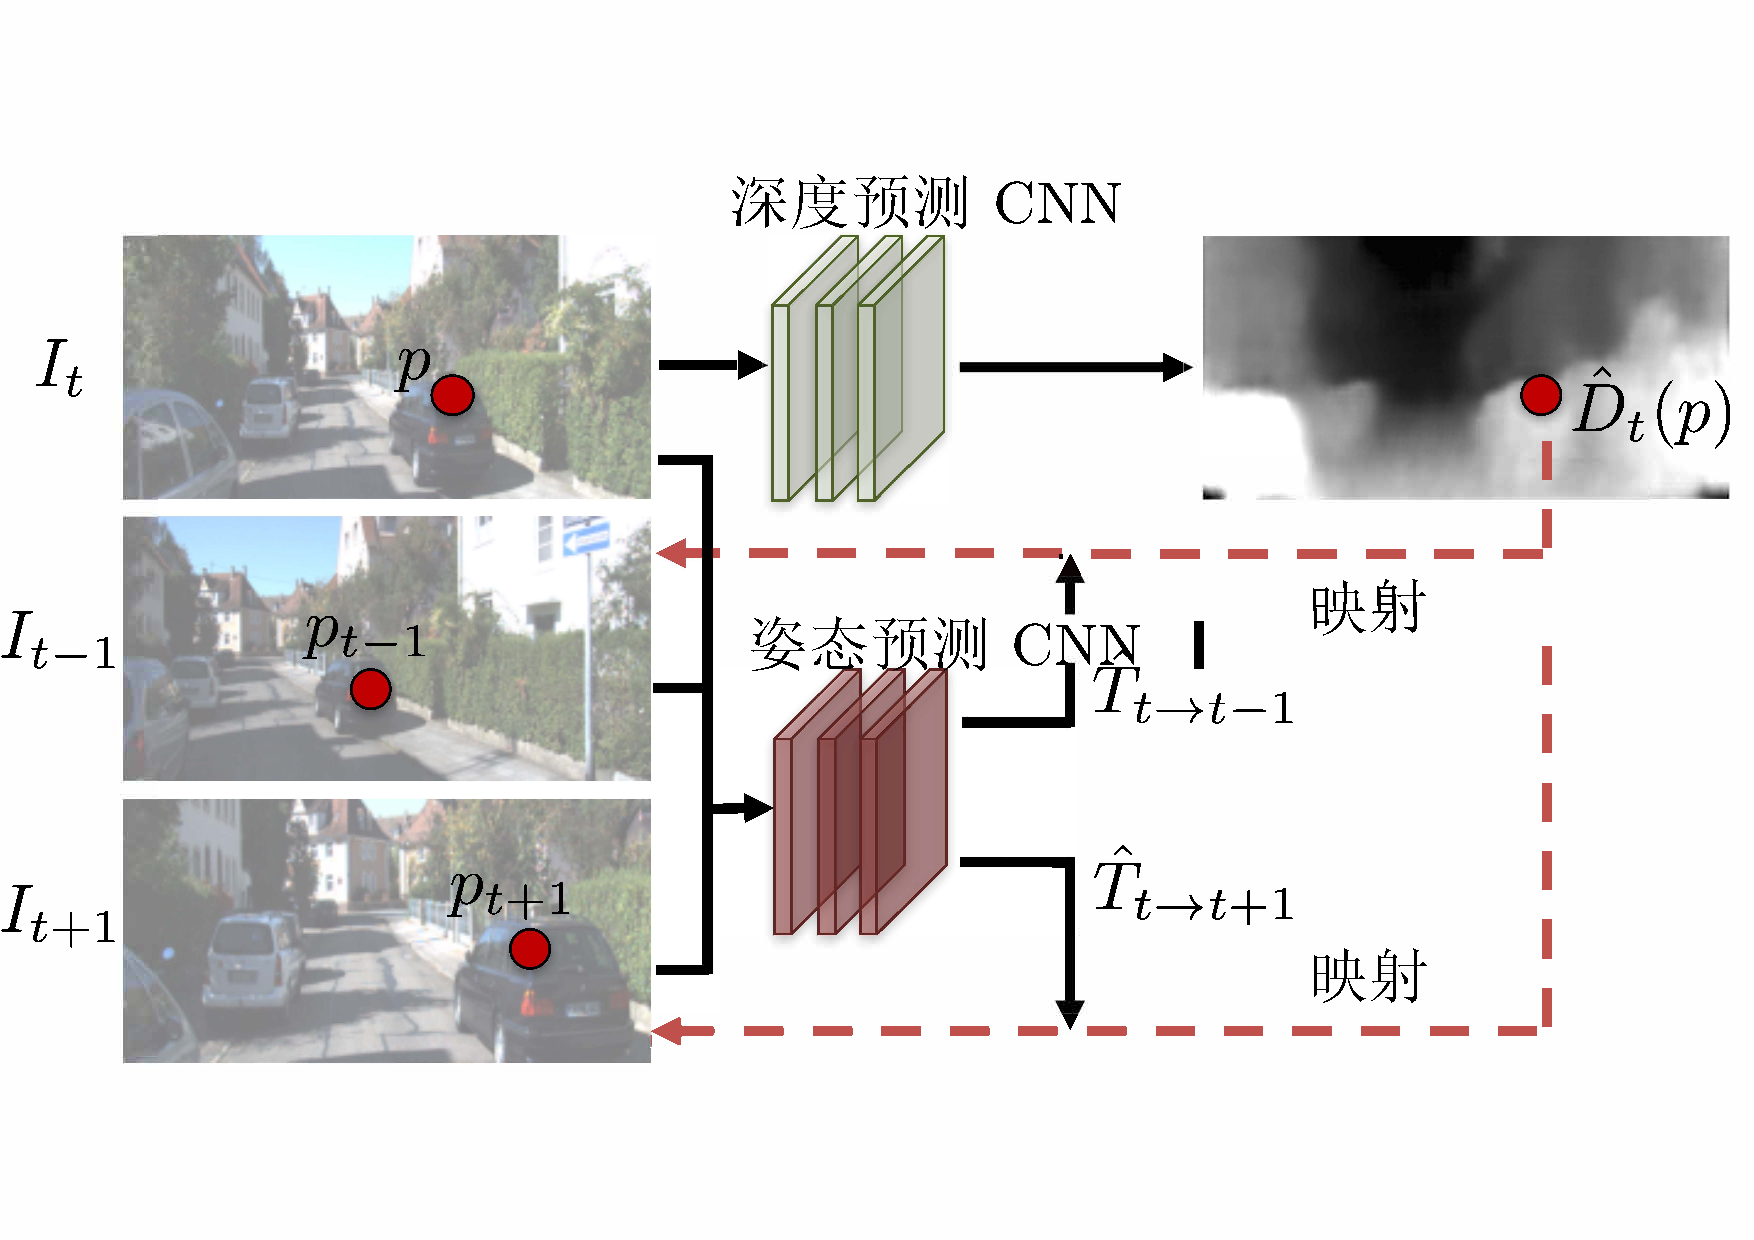
\includegraphics[width=0.9\linewidth]{figure/Sfm.pdf}
    \caption{Zhou等人\cite{zhou2017unsupervised}提出的无监督
    训练框架,可以同时预测相机姿态与深度信息。}
    \label{sfm_zhou}
\end{figure}

Zhou等人\cite{zhou2017unsupervised}提出了一种姿态和深度联合估计的
框架。这种框架利用一段视频作为输入,以视频中的三帧图像为例,
方法使用一个神经网络对中间帧进行深度估计,同时以中间帧和前帧作为
姿态网络的输入,得到一个六自由度的姿态转换矩阵,当获得姿态和深度信息后
中间帧可以重新合成出一张前帧,利用前帧与合成前帧的光度误差,可以
约束整个训练过程,后帧同理。该方法不仅可以同时进行相机的姿态估
计和深度估计,而且不需要任何的数据标注,只需要一段视频即可完成。
在视觉里程估计(VO)和即时定位与建图(SLAM)方向都有很重要的意义。

双目无监督估计\cite{garg2016unsupervised}存在着一些问题:
双目图像并不是完全相同的,左视图和右视图分别有一些各自的盲区;
另外还有遮挡移动等问题会影响预测的结果。
所以针对这些问题Godard等人\cite{Godard2019}提出了一种解决方法:
针对移动和遮挡的问题,设计了一种掩码,
该掩码解决了假设相机在静态场景中移动变化有关的问题。尤其是
一个物体正在以与相机相似的速度移动,
也就是那些在相机坐标系里静
止的物体。这些相对静止的物体的位置在无监督算法的前后帧
几乎没有变化,也即视差为0,理论上应该有无穷大的深度。该
方掩码可以过滤从一帧更改为下一帧时造成误差的像素,
即那些和相机同步运动的像素。
\begin{figure}[tbp]
    \centering
    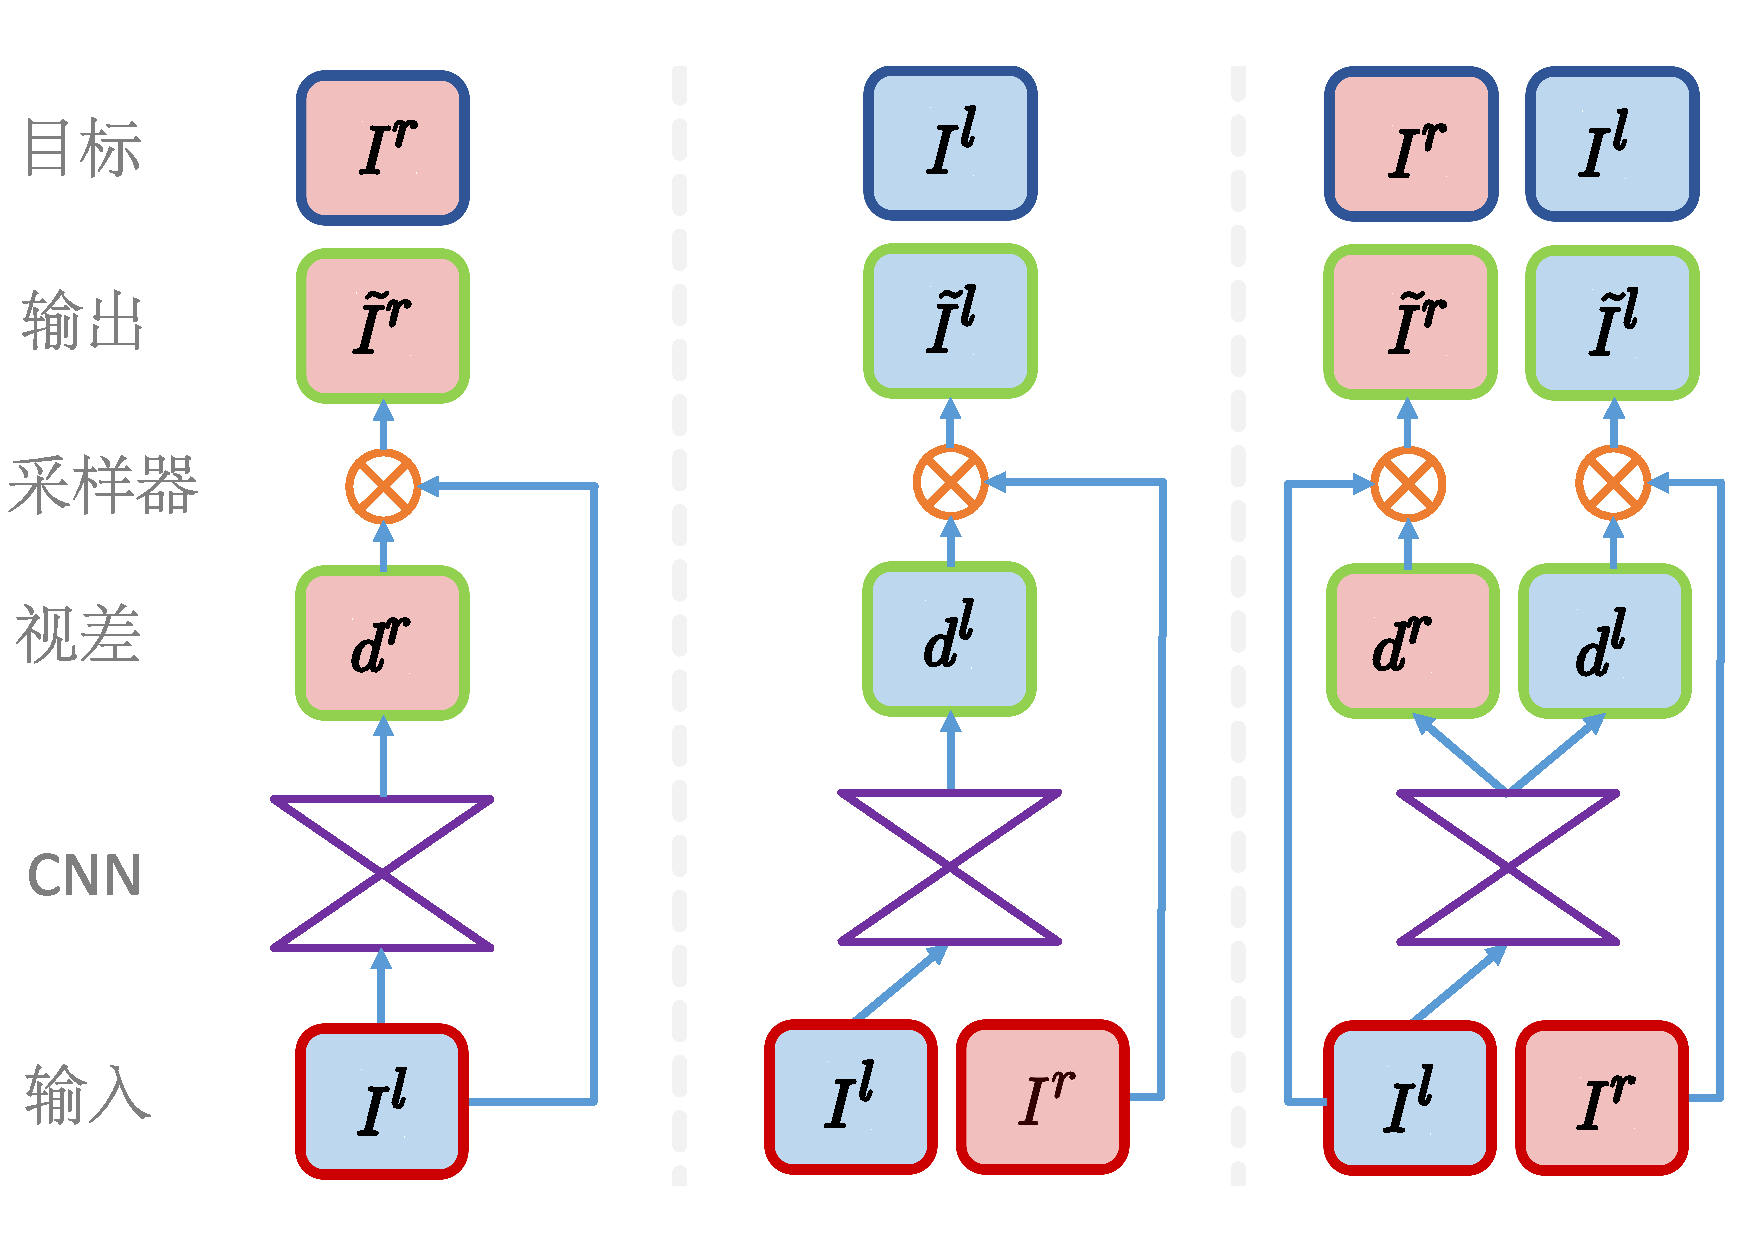
\includegraphics[width=0.7\linewidth]{figure/lr.pdf}
    \caption{Godard等人\cite{Godard2019}根据左右视图的一致性,提出了
    双目无监督框架。}
    \label{Sfm}
\end{figure}
\subsubsection{半监督方法}
%两级标题之间要有过渡性文字。可以通过一段话引出下面的文字
%或者对本章内容概括。论文中凡非正式参考文献以外的资料,
%应以脚注的方式注明\footnote{大家要养成添加脚注的好习惯}。
由于不需要标注数据,无监督方法的性能与有监督方法还有一定的差距。
另外,无监督方法也存在各种各样的问题,例如尺度不一致问题等。
因此,学者们在减少对标注数据的依赖下提出了一种提高估计精度的半监督方法。

Kuznietsov等人\cite{kuznietsov}提出了一种依靠双目图像和雷达点云
数据的半监督预测框架。该框架需要一组双目RGB图像和对应的雷达点云
作为输入。双目图像经过CNN后预测出一对深度图,深度图与稀疏的点云数据在
监督损失函数的约束下趋于一致。同时深度图可以与双目视图中的一张图像
合成出另一视角的观测图像,该图像在无监督损失函数的作用下与
真实的图像趋于一致。
除了这两个损失函数,作者还根据深度图只在物体边缘发生
剧变的特性设计了梯度平滑损失函数。

\section{本文的研究内容与主要工作}

本文的创新点及主要工作如下:
\begin{enumerate}
    \item 针对单目深度估计任务提出了一种基于像素分类的单目深度估计
    框架。该框架在像素级别上生成一系列的备选深度,预测该
    像素上每个备选深度的置信度,如图\ref{Pick}所示。
    \begin{figure*}[htb]
        \centering
        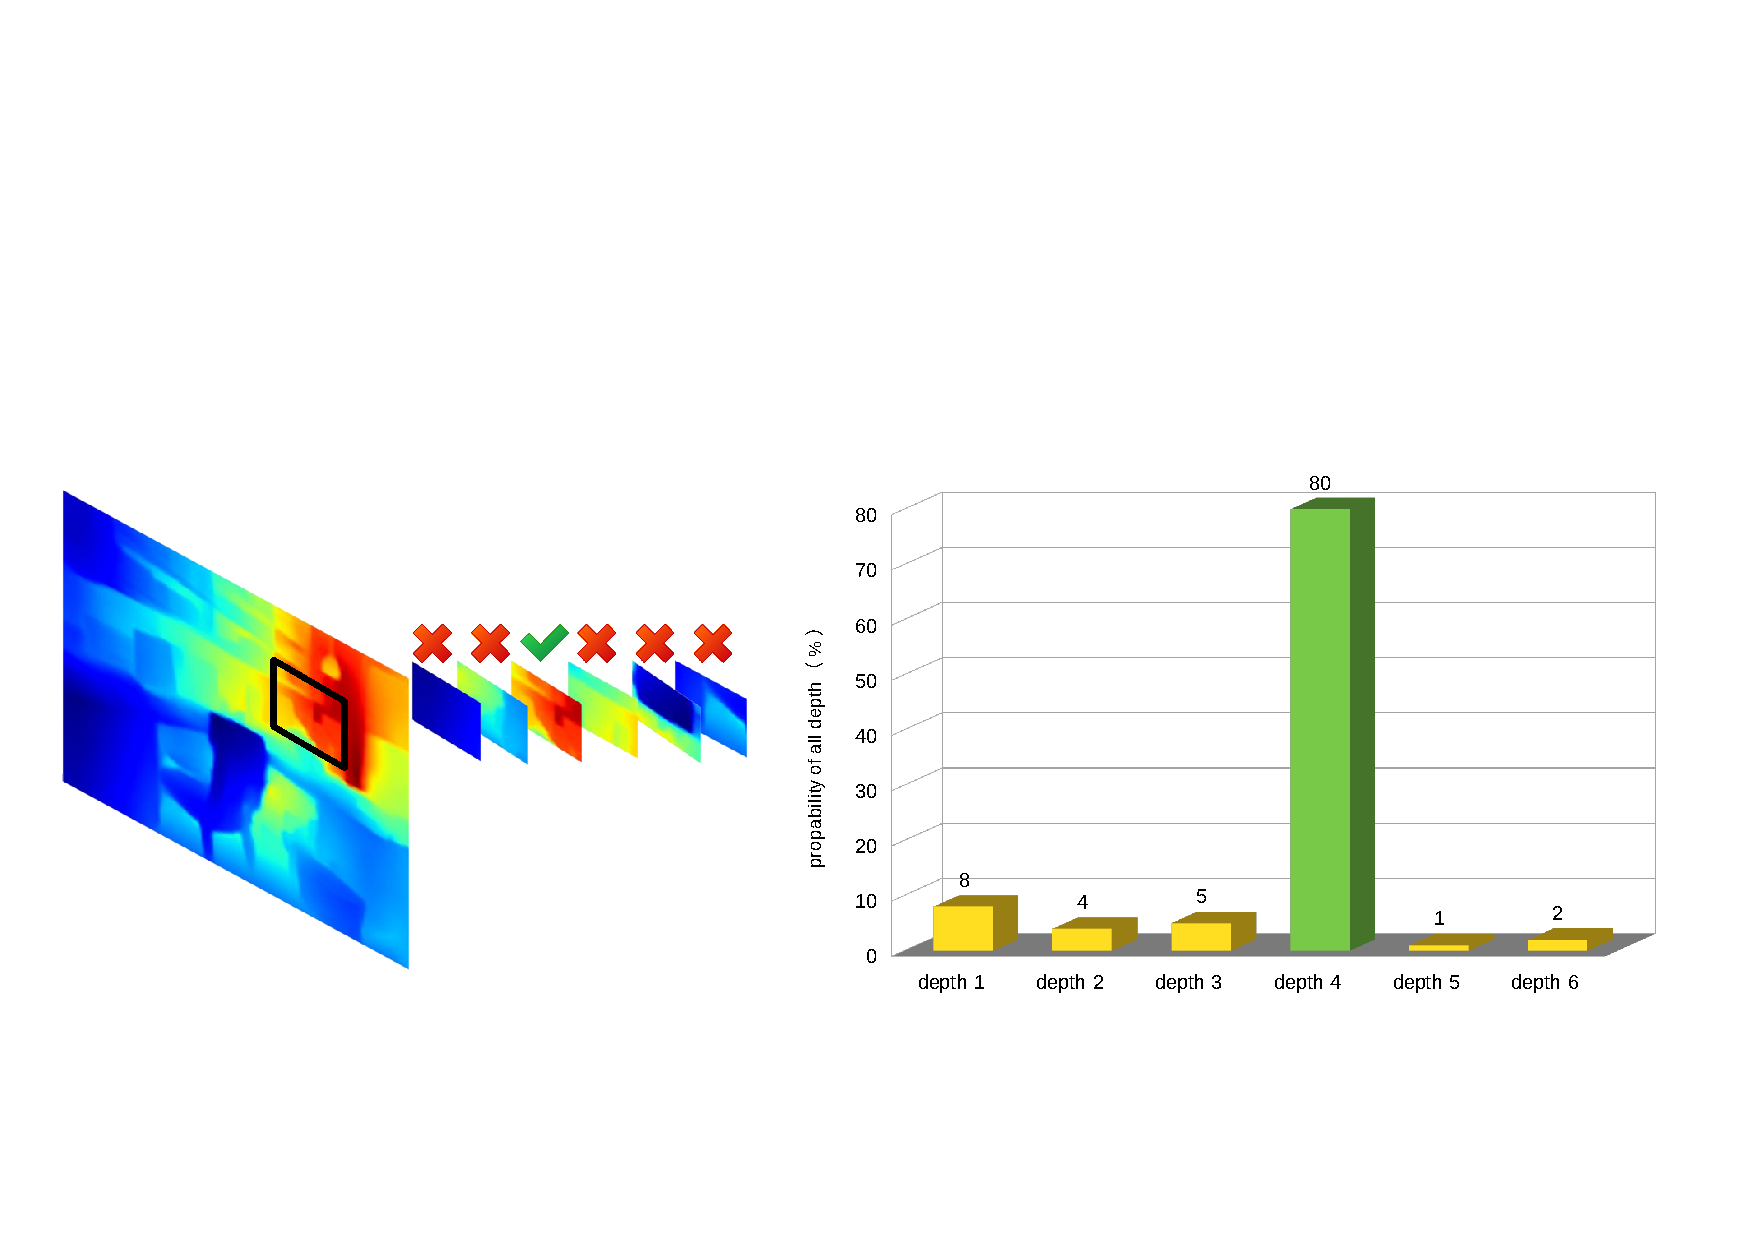
\includegraphics[width=0.9\linewidth]{figure/Pick.pdf}
        \caption{在每个像素位置生成一系列备选像素并计算每个深度的置信度}
        \label{Pick}
    \end{figure*}
    在上采样结构中加入了特征注意力模块(Feature Attention Module),
    该模块在上采样过程中,将短路连接输入的编码端特征图与解码端特征图
    在通道维度内做了不同程度的关注,使得两个信息源有所侧重的重建深度。
    \item 现有算法大多在单一场景进行实验,例如在室外场景数据集训练并且测试,
    或者在单一的室内场景数据集训练和测试。这种算法鲁棒性较差:
    当将室外场景数据集训练的算法应用在室内数据集时表现不佳。
    本文旨在提高算法的泛化能力,
    创造性地将室外数据集合室内数据集结合在一起对单目深度估计进行训练。
    但是预测结果相比单一数据集出现了退化现象。即复杂多样的数据集对
    网络拟合能力和表达能力带来的挑战。
    \item 为了进一步提高网络的拟合能力和表达能力,受到知识蒸馏算法的启发,
    本文提出了一种自蒸馏单目深度估计框架。
    经过实验对比发现,该自蒸馏方法可以有效地解决网络在面临多种数据
    分布时的退化问题。大大提高了网络的表达能力与拟合能力。
    更重要的是该的框架可以应用于所有的端到端编解码网络,
    为后面的融合工作打下了基础。
\end{enumerate}

\section{本文的论文结构与章节安排}

\label{sec:arrangement}
本文共分为五章,各章节内容安排如下:第一章介绍了选题的背景和意义,
按照类别介绍了国内外在单目深度估计的发展现状。并简要描述了
本文的创新点以及工作。因为本文以深度学习算法为基础来进行算法
实现,所以在第二章深度学习算法概述中重点描述本文
使用的卷积神经网络(CNN),以及基于深度学习的单目深度估计
的基础知识:例如常用数据集和评价指标等。
第三章描述了本文提出的基于像素分类单目深度估计方法,该方法是端到端的编解码网络,
在编码端添加了向解码端输入数据的短路连接。在解码端设计了
特征注意力模块,用来对编码端输入的特征和解码端的特征进行
有效地关注,从而提升重建效果。
第四章介绍了提出的自蒸馏学习框架,并进行了实验验证,实验表明
该框架可以有效地解决网络面对复杂数据集的表达能力不足,难以
拟合的问题。
第五章对本文总结反思,审视不足,展望未来工作。

